% Options for packages loaded elsewhere
\PassOptionsToPackage{unicode}{hyperref}
\PassOptionsToPackage{hyphens}{url}
%
\documentclass[
]{article}
\usepackage{amsmath,amssymb}
\usepackage{lmodern}
\usepackage{iftex}
\ifPDFTeX
  \usepackage[T1]{fontenc}
  \usepackage[utf8]{inputenc}
  \usepackage{textcomp} % provide euro and other symbols
\else % if luatex or xetex
  \usepackage{unicode-math}
  \defaultfontfeatures{Scale=MatchLowercase}
  \defaultfontfeatures[\rmfamily]{Ligatures=TeX,Scale=1}
\fi
% Use upquote if available, for straight quotes in verbatim environments
\IfFileExists{upquote.sty}{\usepackage{upquote}}{}
\IfFileExists{microtype.sty}{% use microtype if available
  \usepackage[]{microtype}
  \UseMicrotypeSet[protrusion]{basicmath} % disable protrusion for tt fonts
}{}
\makeatletter
\@ifundefined{KOMAClassName}{% if non-KOMA class
  \IfFileExists{parskip.sty}{%
    \usepackage{parskip}
  }{% else
    \setlength{\parindent}{0pt}
    \setlength{\parskip}{6pt plus 2pt minus 1pt}}
}{% if KOMA class
  \KOMAoptions{parskip=half}}
\makeatother
\usepackage{xcolor}
\usepackage[margin=1in]{geometry}
\usepackage{graphicx}
\makeatletter
\def\maxwidth{\ifdim\Gin@nat@width>\linewidth\linewidth\else\Gin@nat@width\fi}
\def\maxheight{\ifdim\Gin@nat@height>\textheight\textheight\else\Gin@nat@height\fi}
\makeatother
% Scale images if necessary, so that they will not overflow the page
% margins by default, and it is still possible to overwrite the defaults
% using explicit options in \includegraphics[width, height, ...]{}
\setkeys{Gin}{width=\maxwidth,height=\maxheight,keepaspectratio}
% Set default figure placement to htbp
\makeatletter
\def\fps@figure{htbp}
\makeatother
\setlength{\emergencystretch}{3em} % prevent overfull lines
\providecommand{\tightlist}{%
  \setlength{\itemsep}{0pt}\setlength{\parskip}{0pt}}
\setcounter{secnumdepth}{-\maxdimen} % remove section numbering
\usepackage{caption}
\usepackage{subfig}
\usepackage{float}
\captionsetup[figure]{labelformat=empty}
\captionsetup[table]{labelformat=empty}
\usepackage{booktabs}
\usepackage{longtable}
\usepackage{array}
\usepackage{multirow}
\usepackage{wrapfig}
\usepackage{float}
\usepackage{colortbl}
\usepackage{pdflscape}
\usepackage{tabu}
\usepackage{threeparttable}
\usepackage{threeparttablex}
\usepackage[normalem]{ulem}
\usepackage{makecell}
\usepackage{xcolor}
\ifLuaTeX
  \usepackage{selnolig}  % disable illegal ligatures
\fi
\IfFileExists{bookmark.sty}{\usepackage{bookmark}}{\usepackage{hyperref}}
\IfFileExists{xurl.sty}{\usepackage{xurl}}{} % add URL line breaks if available
\urlstyle{same} % disable monospaced font for URLs
\hypersetup{
  pdftitle={Water Withdrawal Report for the Lower Savannah-Salkehatchie Basin (2022)},
  pdfauthor={Priyanka More},
  hidelinks,
  pdfcreator={LaTeX via pandoc}}

\title{Water Withdrawal Report for the Lower Savannah-Salkehatchie Basin
(2022)}
\author{Priyanka More}
\date{2024-05-16}

\begin{document}
\maketitle

~~~~~~This report summarizes reported water withdrawals in the Lower
Savannah-Salkehatchie River basin for the year 2022, provided by the
South Carolina Department of Health and Environmental Control (SCDHEC)
through the Surface Water Withdrawal, Permitting, Use and Reporting Act
and the Groundwater Use and Reporting Act, both administered by SCDHEC.
The SCDHEC maintains a water-use database for all the registered and
permitted users of all major categories (Table 1) in the state that are
required to report their water withdrawals for the active months and
years (SCDHEC Water Use Report, 2020)\(^1\).\\
\hspace*{0.333em}\hspace*{0.333em}\hspace*{0.333em}\hspace*{0.333em}\hspace*{0.333em}\hspace*{0.333em}In
this report, the term ``withdrawal'' refers to the surface or
groundwater withdrawn by a water user/ facility from a surface water
source (river, lake, pond) or groundwater source (aquifer). SCDHEC has
water withdrawal data in million gallons per month (MGM), however, for
this annual report, the monthly withdrawals were summed for the required
year and averaged in million gallons per day (MGD).

\begin{table}[!h]
\centering
\caption{\label{tab:water-use-cat-description}\textbf{Table 1.} Description of water use categories}
\centering
\begin{tabular}[t]{l>{\raggedright\arraybackslash}p{12 cm}}
\toprule
\multicolumn{1}{c}{Category} & \multicolumn{1}{>{\centering\arraybackslash}p{12 cm}}{Description}\\
\midrule
Thermoelectric Power & Water used in generating electricity from fossil fuel (coal, oil, natural gas), geothermal, biomass, soild waste, or nuclear energy.\\
Hydroelectric Power & Water used in generating electricity where turbine generators are driven by falling water.\\
Water Supply & Water withdrawn by public and private water suppliers and conveyed to users or groups of users. Water Suppliers provide water for a variety of uses including domestic, commercial, industrial and public water use.\\
Industry & Water used for commercial and industrial purposes, including fabrication, processing, washing, in-plant conveyance and cooling.\\
Agriculture & Water used for agricultural and landscaping purposes, including turf farming and livestock management.\\
Golf Course & Water used to maintain golf course turf, including tee boxes, fairways, putting greens, associated practice areas and periphery aesthetic landscaping.\\
Mining & Water used for in conjunction with surface or subsurface mining of minerals or natural materials.\\
Aquaculture & Water used for raising, farming, and/or harvesting organisms that live in water, such as shrimp, fish, and other vegetal matter (seaweed).\\
\bottomrule
\end{tabular}
\end{table}

\begin{figure}
\centering
\includegraphics{Lower_Savannah_Salkehatchie_files/figure-latex/LSS-map-1.pdf}
\caption{\textbf{Figure 1.} Major river basins in South Carolina,
highlighting the Lower Savannah-Salkehatchie basin.}
\end{figure}

\hypertarget{summary-of-water-withdrawals-excluding-hydroelectric-power}{%
\subsection{1.1 Summary of Water Withdrawals, Excluding Hydroelectric
Power}\label{summary-of-water-withdrawals-excluding-hydroelectric-power}}

~~~~~~Water used for Hydroelectric Power generation is returned directly
to the river from which it was withdrawn and is, therefore, omitted from
this analysis. After excluding water withdrawals for Hydroelectric
Power, the Lower Savannah-Salkehatchie basin (Fig. 1) had the seventh
highest total water withdrawals among the eight major river basins in
the State (Table 2). In 2022, 228.0 million gallons per day (MGD) were
withdrawn from the Lower Savannah-Salkehatchie basin, accounting for 3.9
percent of the total amount of water used in the State. The basin had
the second highest groundwater withdrawals (73.0 MGD), accounting for
26.1 percent of the total amount of groundwater used in the State, and
the seventh highest surface water withdrawals (155.0 MGD), accounting
for 2.8 percent of the total amount of surface water used in the State
(Table 2).

\begin{table}[!h]
\centering
\caption{\label{tab:Table_2}\textbf{Table 2.} 2022 Water withdrawals excluding Hydroelectric Power in the eight major river basins by source}
\centering
\begin{tabular}[t]{>{\raggedright\arraybackslash}p{2 cm}>{\raggedleft\arraybackslash}p{2 cm}>{\raggedleft\arraybackslash}p{2 cm}>{\raggedleft\arraybackslash}p{2 cm}>{\raggedleft\arraybackslash}p{2 cm}>{\raggedleft\arraybackslash}p{2 cm}>{\raggedleft\arraybackslash}p{2 cm}}
\toprule
\multicolumn{1}{c}{ } & \multicolumn{2}{c}{Groundwater} & \multicolumn{2}{c}{Surface Water} & \multicolumn{2}{c}{Total} \\
\cmidrule(l{3pt}r{3pt}){2-3} \cmidrule(l{3pt}r{3pt}){4-5} \cmidrule(l{3pt}r{3pt}){6-7}
Basin & Withdrawals (MGD) & $\%$ of total withdrawals & Withdrawals (MGD) & $\%$ of total withdrawals & Withdrawals (MGD) & $\%$ of total withdrawals\\
\midrule
Broad & 0.5 & 0.2 & 835.0 & 14.9 & 835.5 & 14.2\\
Catawba & 6.3 & 2.3 & 257.7 & 4.6 & 264.0 & 4.5\\
Edisto & 64.0 & 22.9 & 64.1 & 1.1 & 128.1 & 2.2\\
Lower Savannah-Salkehatchie & 73.0 & 26.1 & 155.0 & 2.8 & 228.0 & 3.9\\
Pee Dee & 106.8 & 38.2 & 803.7 & 14.3 & 910.5 & 15.5\\
Saluda & 0.2 & 0.1 & 244.0 & 4.4 & 244.3 & 4.1\\
Santee & 28.4 & 10.1 & 482.6 & 8.6 & 511.0 & 8.7\\
Upper Savannah & 0.4 & 0.1 & 2,765.5 & 49.3 & 2,765.9 & 47.0\\
\midrule\\
Total & 279.8 & 100.0 & 5,607.8 & 100.0 & 5,887.6 & 100.0\\
\bottomrule
\end{tabular}
\end{table}

\begin{table}[!h]
\centering
\caption{\label{tab:summary-source-no-PH}\textbf{Table 3.} 2022 Water withdrawals excluding Hydroelectric Power in the Lower Savannah-Salkehatchie basin by source }
\centering
\begin{tabular}[t]{l>{\raggedleft\arraybackslash}m{3 cm}>{\raggedleft\arraybackslash}m{3 cm}}
\toprule
Source & Withdrawals (MGD) & $\%$ of total withdrawals\\
\midrule
Groundwater & 73 & 32\\
Surface Water & 155 & 68\\
\midrule\\
Total & 228 & 100\\
\bottomrule
\end{tabular}
\end{table}

~~~~~~Of the 228.0 MGD withdrawn in the Lower Savannah-Salkehatchie
basin in 2022, surface water sources accounted for 68.0 percent (155.0
MGD) and groundwater sources for 32.0 percent (73.0 MGD) (Table 3).
Among the water-use categories, Thermoelectric Power used, by far, the
most water (89.7 MGD) accounting for 39.3 percent of the total, followed
by Water Supply (73.4 MGD; 32.2 percent) and Agriculture (34.2 MGD; 15.0
percent) (Table 4). The remaining water-use categories used much lesser
amounts---Industry accounting for 10.9 percent (24.8 MGD), Golf Course
for 2.0 percent (4.7 MGD), Aquaculture for 0.5 percent (1.2 MGD), and
Other for 0.0 percent (0.1 MGD) (Table 4; Fig. 2).

~~~~~~Of the 155.0 MGD withdrawn from surface water sources in the Lower
Savannah-Salkehatchie basin, Thermoelectric Power accounted for 57.6
percent (89.3 MGD), followed by Water Supply (39.2 MGD; 25.3 percent)
and Industry (21.2 MGD; 13.6 percent). The remaining water use
categories had much smaller withdrawals with Agriculture accounting for
1.8 percent (2.7 MGD), Golf Course for 1.1 percent (1.7 MGD), and
Aquaculture for 0.6 percent (0.9 MGD) (Table 4; Fig. 2).

~~~~~~Of the 73.0 MGD withdrawn from groundwater sources in the Lower
Savannah-Salkehatchie basin, Water Supply had highest withdrawals,
accounting for 46.8 percent (34.2 MGD), followed by Agriculture (31.5
MGD; 43.2 percent) and Industry (3.6 MGD; 4.9 percent). The remaining
water use categories had much smaller withdrawals with Golf Course
accounting for 4.1 percent (3.0 MGD), Thermoelectric Power for 0.5
percent (0.4 MGD), Aquaculture for 0.4 percent (0.3 MGD), and Other for
0.1 percent (0.1 MGD) (Table 4; Fig.2).

\begin{table}[!h]
\centering
\caption{\label{tab:summary-pie-chart-cat-no-ph}\textbf{Table 4.} 2022 Water withdrawals excluding Hydroelectric Power in the Lower Savannah-Salkehatchie basin by category and source }
\centering
\begin{tabular}[t]{l>{\raggedleft\arraybackslash}p{2 cm}>{\raggedleft\arraybackslash}p{2 cm}>{\raggedleft\arraybackslash}p{2 cm}>{\raggedleft\arraybackslash}p{2 cm}>{\raggedleft\arraybackslash}p{2 cm}>{\raggedleft\arraybackslash}p{2 cm}}
\toprule
\multicolumn{1}{c}{ } & \multicolumn{2}{c}{Groundwater} & \multicolumn{2}{c}{Surface Water} & \multicolumn{2}{c}{Total} \\
\cmidrule(l{3pt}r{3pt}){2-3} \cmidrule(l{3pt}r{3pt}){4-5} \cmidrule(l{3pt}r{3pt}){6-7}
Category & Withdrawals (MGD) & $\%$ of total withdrawals & Withdrawals (MGD) & $\%$ of total withdrawals & Withdrawals (MGD) & $\%$ of total withdrawals\\
\midrule
Agriculture & 31.5 & 43.2 & 2.7 & 1.8 & 34.2 & 15.0\\
Aquaculture & 0.3 & 0.4 & 0.9 & 0.6 & 1.2 & 0.5\\
Golf Course & 3.0 & 4.1 & 1.7 & 1.1 & 4.7 & 2.0\\
Industry & 3.6 & 4.9 & 21.2 & 13.6 & 24.8 & 10.9\\
Other & 0.1 & 0.1 & NA & NA & 0.1 & 0.0\\
Thermoelectric & 0.4 & 0.5 & 89.3 & 57.6 & 89.7 & 39.3\\
Water Supply & 34.2 & 46.8 & 39.2 & 25.3 & 73.4 & 32.2\\
\midrule\\
Total & 73.0 & 100.0 & 155.0 & 100.0 & 228.0 & 100.0\\
\bottomrule
\end{tabular}
\end{table}

\begin{figure}[H]

{\centering 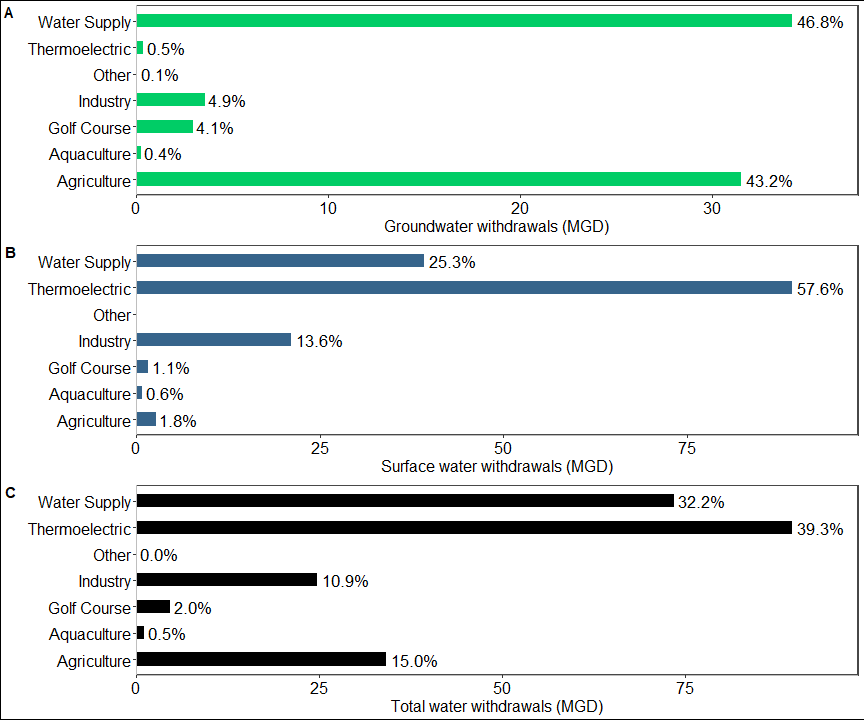
\includegraphics{LSS_figures/combine-bar-plots-noPH-1} 

}

\caption{\textbf{Figure 2.} 2022 Water withdrawals excluding Hydroelectric Power in the Lower Savannah-Salkehatchie basin by category and source. Groundwater \textbf{(A)}, Surface Water \textbf{(B)}, and Total \textbf{(C)}.}\label{fig:combine-bar-plots-noPH}
\end{figure}

\newpage

\hypertarget{summary-of-water-withdrawals-excluding-hydroelectric-power-and-thermoelectric-power}{%
\subsection{1.2 Summary of Water Withdrawals, Excluding Hydroelectric
Power and Thermoelectric
Power}\label{summary-of-water-withdrawals-excluding-hydroelectric-power-and-thermoelectric-power}}

~~~~~~Electrical power generation has high water use in the State (South
Carolina State Water Assessment, 2009)\(^2\), which tends to overshadow
the use of the other major water use categories. The relative proportion
of water used by the remaining categories can be clearly illustrated and
understood by excluding water used for power generation. For example, on
excluding the water used in the State for Hydroelectric and
Thermoelectric Power, total water withdrawals in the Lower
Savannah-Salkehatchie basin ranked fourth highest among the eight river
basins, accounting for 11.9 percent (MGD) of the total water withdrawn
in the State (Table 5). On excluding water used for power generation,
the Lower Savannah-Salkehatchie basin had the seventh highest amount of
surface water used in the State (65.7 MGD; 7.4 percent) and the second
highest amount of groundwater withdrawn (72.6 MGD; 26.1 percent) (Table
5).

\begin{table}[!h]
\centering
\caption{\label{tab:Table_5}\textbf{Table 5.} 2022 Water withdrawals excluding Hydroelectric and Thermoelectric Power in the eight major river basins by source }
\centering
\begin{tabular}[t]{>{\raggedright\arraybackslash}p{2 cm}>{\raggedleft\arraybackslash}p{2 cm}>{\raggedleft\arraybackslash}p{2 cm}>{\raggedleft\arraybackslash}p{2 cm}>{\raggedleft\arraybackslash}p{2 cm}>{\raggedleft\arraybackslash}p{2 cm}>{\raggedleft\arraybackslash}p{2 cm}}
\toprule
\multicolumn{1}{c}{ } & \multicolumn{2}{c}{Groundwater} & \multicolumn{2}{c}{Surface Water} & \multicolumn{2}{c}{Total} \\
\cmidrule(l{3pt}r{3pt}){2-3} \cmidrule(l{3pt}r{3pt}){4-5} \cmidrule(l{3pt}r{3pt}){6-7}
Basin & Withdrawals (MGD) & $\%$ of total withdrawals & Withdrawals (MGD) & $\%$ of total withdrawals & Withdrawals (MGD) & $\%$ of total withdrawals\\
\midrule
Broad & 0.5 & 0.2 & 107.8 & 12.2 & 108.3 & 9.4\\
Catawba & 6.3 & 2.3 & 122.9 & 13.9 & 129.3 & 11.2\\
Edisto & 60.7 & 22.1 & 64.1 & 7.3 & 124.8 & 10.8\\
Lower Savannah-Salkehatchie & 72.6 & 26.4 & 65.7 & 7.4 & 138.4 & 11.9\\
Pee Dee & 105.7 & 38.4 & 149.7 & 16.9 & 255.4 & 22.0\\
Saluda & 0.2 & 0.1 & 148.5 & 16.8 & 148.7 & 12.8\\
Santee & 28.4 & 10.3 & 151.3 & 17.1 & 179.7 & 15.5\\
Upper Savannah & 0.4 & 0.1 & 73.1 & 8.3 & 73.5 & 6.3\\
\midrule\\
Total & 275.2 & 100.0 & 883.2 & 100.0 & 1,158.3 & 100.0\\
\bottomrule
\end{tabular}
\end{table}

\begin{table}[!h]
\centering
\caption{\label{tab:summary-source-no-power}\textbf{Table 6.} 2022 Water withdrawals excluding Hydroelectric and Thermoelectric Power in the Lower Savannah-Salkehatchie basin by source}
\centering
\begin{tabular}[t]{l>{\raggedleft\arraybackslash}m{3 cm}>{\raggedleft\arraybackslash}m{3 cm}}
\toprule
Source & Withdrawals (MGD) & $\%$ of total withdrawals\\
\midrule
Groundwater & 72.6 & 52.5\\
Surface Water & 65.7 & 47.5\\
\midrule\\
Total & 138.4 & 100.0\\
\bottomrule
\end{tabular}
\end{table}

~~~~~~Of the 138.4 MGD withdrawn in the Lower Savannah-Salkehatchie
basin in 2022. Surface water sources accounted for 47.5 percent (65.7
MGD) and groundwater sources for 52.5 percent (72.6 MGD) (Table 6).
Among the water-use categories, Water Supply used, by far, the most
water (73.4 MGD) accounting for 53.1 percent of the total, followed by
Agriculture (34.2 MGD; 24.7 percent) and Industry (24.8 MGD; 17.9
percent) (Table 7). The remaining water-use categories used much lesser
amounts---Golf Course accounting for 3.4 percent (4.7 MGD), Aquaculture
for 0.86 percent (1.2 MGD), and Other for 0.05 percent (0.1 MGD)(Table
7; Fig. 3).

~~~~~~Of the 65.7 MGD withdrawn from surface water sources in the Lower
Savannah-Salkehatchie basin, Water Supply accounted for 59.7 percent
(39.2 MGD), followed by Industry (21.2 MGD; 32.2 percent) and
Agriculture (2.7 MGD; 4.1 percent). The remaining water use categories
had much smaller withdrawals with Golf Course accounting for 2.6 percent
(1.7 MGD) and Aquaculture for 1.40 percent (0.9 MGD) (Table 7; Fig. 3).

~~~~~~Of the 72.6 MGD withdrawn from groundwater sources in the Lower
Savannah-Salkehatchie basin, Water Supply had highest withdrawals,
accounting for 47.1 percent (34.2 MGD), followed by Agriculture (31.5
MGD; 43.4 percent), followed by Industry (3.6 MGD; 5.0 percent), Golf
Course (3.0 MGD; 4.1 percent), and Aquaculture (0.3 MGD; 0.4 percent)
(Table 7; Fig.3).

\begin{table}[!h]
\centering
\caption{\label{tab:US-source-cat-no-power-table}\textbf{Table 7.} 2022 Water withdrawals excluding Hydroelectric and Thermoelectric Power in the Lower Savannah-Salkehatchie basin by category and source}
\centering
\begin{tabular}[t]{l>{\raggedleft\arraybackslash}p{2 cm}>{\raggedleft\arraybackslash}p{2 cm}>{\raggedleft\arraybackslash}p{2 cm}>{\raggedleft\arraybackslash}p{2 cm}>{\raggedleft\arraybackslash}p{2 cm}>{\raggedleft\arraybackslash}p{2 cm}}
\toprule
\multicolumn{1}{c}{ } & \multicolumn{2}{c}{Groundwater} & \multicolumn{2}{c}{Surface Water} & \multicolumn{2}{c}{Total} \\
\cmidrule(l{3pt}r{3pt}){2-3} \cmidrule(l{3pt}r{3pt}){4-5} \cmidrule(l{3pt}r{3pt}){6-7}
Category & Withdrawals (MGD) & $\%$ of total withdrawals & Withdrawals (MGD) & $\%$ of total withdrawals & Withdrawals (MGD) & $\%$ of total withdrawals\\
\midrule
Agriculture & 31.5 & 43.4 & 2.7 & 4.1 & 34.2 & 24.7\\
Aquaculture & 0.3 & 0.4 & 0.9 & 1.4 & 1.2 & 0.9\\
Golf Course & 3.0 & 4.1 & 1.7 & 2.6 & 4.7 & 3.4\\
Industry & 3.6 & 5.0 & 21.2 & 32.2 & 24.8 & 17.9\\
Other & 0.1 & 0.1 & NA & NA & 0.1 & 0.1\\
Water Supply & 34.2 & 47.1 & 39.2 & 59.7 & 73.4 & 53.1\\
\midrule\\
Total & 72.6 & 100.0 & 65.7 & 100.0 & 138.4 & 100.0\\
\bottomrule
\end{tabular}
\end{table}

\begin{figure}[H]

{\centering 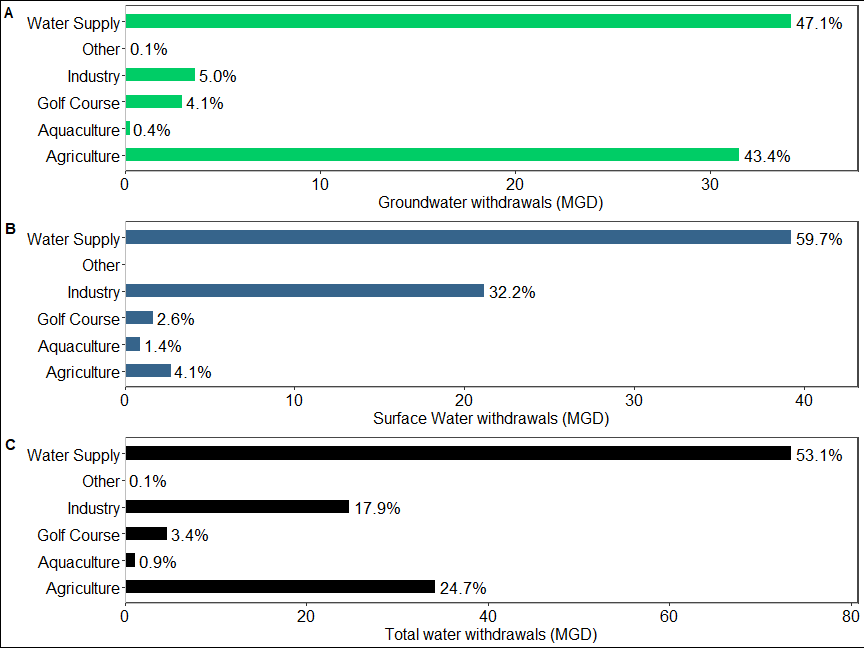
\includegraphics{LSS_figures/combine-bar-plots-nopower-1} 

}

\caption{\textbf{Figure 3.} 2022 Water withdrawals excluding Hydroelectric and Thermoelectric Power in the Lower Savannah-Salkehatchie basin by category and source, Groundwater \textbf{(A)}, Surface Water \textbf{(B)}, and Total \textbf{(C)}.}\label{fig:combine-bar-plots-nopower}
\end{figure}

\newpage

\hypertarget{appendix-a.-water-withdrawal-trends-by-category-and-source-2011-2022}{%
\section{Appendix A. Water Withdrawal Trends by Category and Source
(2011-2022)}\label{appendix-a.-water-withdrawal-trends-by-category-and-source-2011-2022}}

\hypertarget{a.1-limitations-of-the-scdhec-database}{%
\subsection{A.1 Limitations of the SCDHEC
Database}\label{a.1-limitations-of-the-scdhec-database}}

~~~~~~Although the quality of water-use data significantly improved
after 2000, the database is not a complete and accurate representation
of total water withdrawals in the state. Limitations of the SCDHEC
database include:

\begin{enumerate}
\def\labelenumi{\arabic{enumi}.}
\tightlist
\item
  Withdrawals from private domestic wells, small surface water
  irrigation ponds, and any other water withdrawals less than the
  reporting threshold of 3 MGM are excluded from the SCDHEC's water-use
  database (SCDHEC Water Use Report, 2020)\(^1\).
\item
  After passing of the South Carolina Surface Water Withdrawal,
  Permitting, Use, and Reporting Act in 2011, several facilities
  withdrawing less than the threshold value were not required to report
  their withdrawals to SCDHEC.
\item
  Errors in reported water withdrawals or errors introduced during data
  input.
\item
  Some users fail to add metadata such as longitude, latitude, county,
  and basin information for a surface water intake or groundwater well
  withdrawal. This can lead to some inaccuracies in the dataset.
\item
  Increasing trends in reported water withdrawals for some categories
  (Agriculture, for example) may in part be due to increased reporting
  compliance over the analysis period (2011 - 2022).
\end{enumerate}

Owing to the above limitations, caution is warranted when interpreting
trends in reported withdrawals from the SCDHEC water-use database.

\hypertarget{a.2-water-withdrawal-for-all-categories-combined-excluding-hydroelectric-power}{%
\subsection{A.2 Water Withdrawal for All Categories Combined, Excluding
Hydroelectric
Power}\label{a.2-water-withdrawal-for-all-categories-combined-excluding-hydroelectric-power}}

\begin{figure}[H]

{\centering 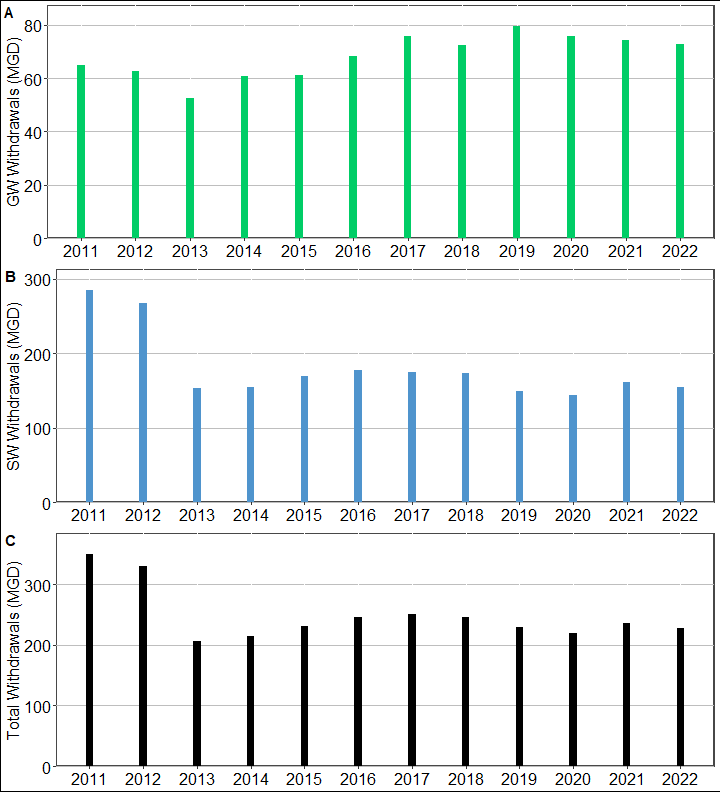
\includegraphics{LSS_figures/trend-bar-plot-all_cat_noPH-1} 

}

\caption{\textbf{Figure A1.} Annual water withdrawals excluding Hydroelectric Power in the Lower Savannah-Salkehatchie basin for remaining categories combined and by source. Groundwater (GW) \textbf{(A)}, Surface Water (SW) \textbf{(B)}, and Total \textbf {(C)}.}\label{fig:trend-bar-plot-all_cat_noPH}
\end{figure}

\hypertarget{a.3-water-withdrawal-for-all-categories-combined-excluding-hydroelectric-and-thermoelectric-power}{%
\subsection{A.3 Water Withdrawal for All Categories Combined, Excluding
Hydroelectric and Thermoelectric
Power}\label{a.3-water-withdrawal-for-all-categories-combined-excluding-hydroelectric-and-thermoelectric-power}}

\begin{figure}[H]

{\centering 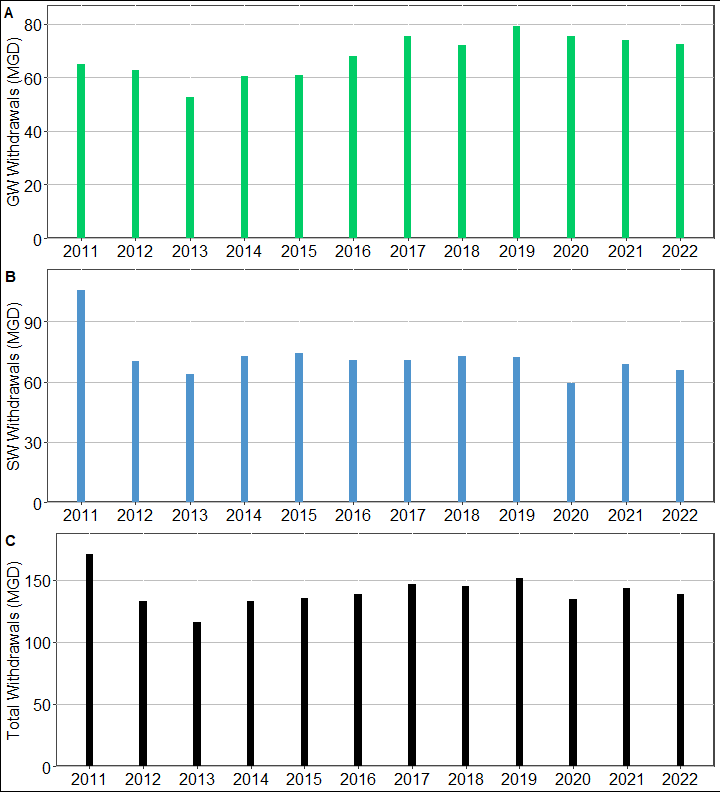
\includegraphics{LSS_figures/trend-bar-plot-all_cat_nopower-1} 

}

\caption{\textbf{Figure A2.} Annual water withdrawals excluding Hydroelectric and Thermoelectric Power in the Lower Savannah-Salkehatchie basin for remaining categories combined and by source. Groundwater (GW) \textbf{(A)}, Surface Water (SW) \textbf{(B)}, and Total \textbf {(C)}.}\label{fig:trend-bar-plot-all_cat_nopower}
\end{figure}

\hypertarget{a.4-water-withdrawal-for-thermoelectric-power}{%
\subsection{A.4 Water Withdrawal for Thermoelectric
Power}\label{a.4-water-withdrawal-for-thermoelectric-power}}

\begin{figure}[H]

{\centering 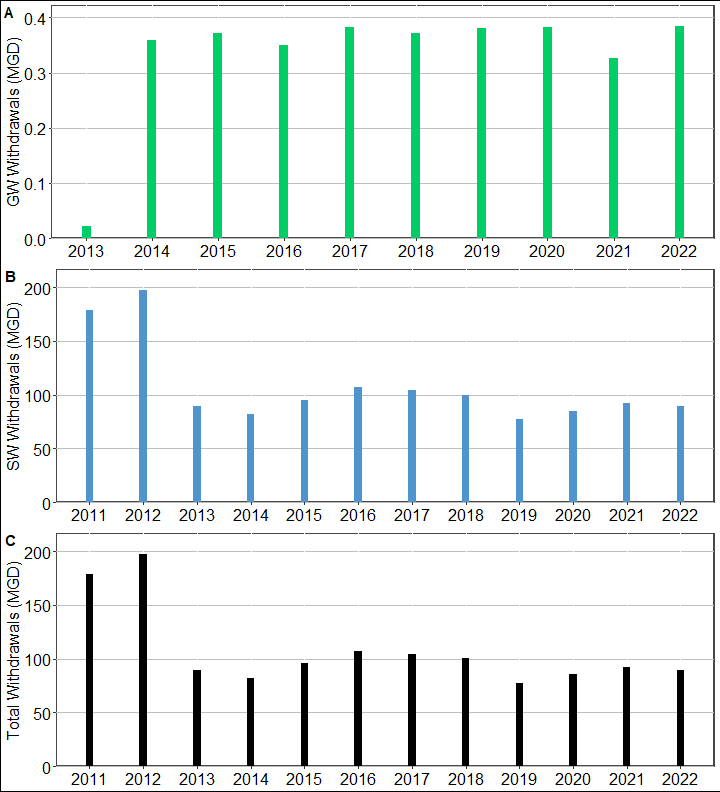
\includegraphics{LSS_figures/trend-TH_bar-plot-1} 

}

\caption{\textbf{Figure A3.} Annual water withdrawals in the Lower Savannah-Salkehatchie for Thermoelectric Power by source. Groundwater (GW) \textbf{(A)}, Surface Water (SW) \textbf{(B)}, and Total \textbf {(C)}.}\label{fig:trend-TH_bar-plot}
\end{figure}

\hypertarget{a.5-water-withdrawal-for-water-supply}{%
\subsection{A.5 Water Withdrawal for Water
Supply}\label{a.5-water-withdrawal-for-water-supply}}

\begin{figure}[H]

{\centering 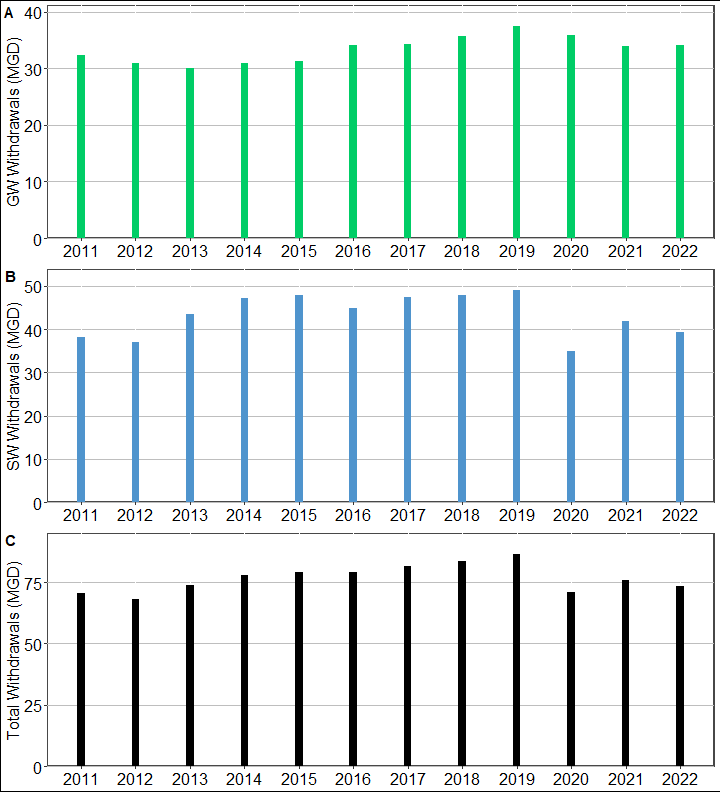
\includegraphics{LSS_figures/trend-WS_bar-plot-1} 

}

\caption{\textbf{Figure A4.} Annual water withdrawals in the Lower Savannah-Salkehatchie basin for Water Supply by source. Groundwater (GW) \textbf{(A)}, Surface Water (SW) \textbf{(B)}, and Total \textbf {(C)}.}\label{fig:trend-WS_bar-plot}
\end{figure}

\hypertarget{a.6-water-withdrawal-for-industry}{%
\subsection{A.6 Water Withdrawal for
Industry}\label{a.6-water-withdrawal-for-industry}}

\begin{figure}[H]

{\centering 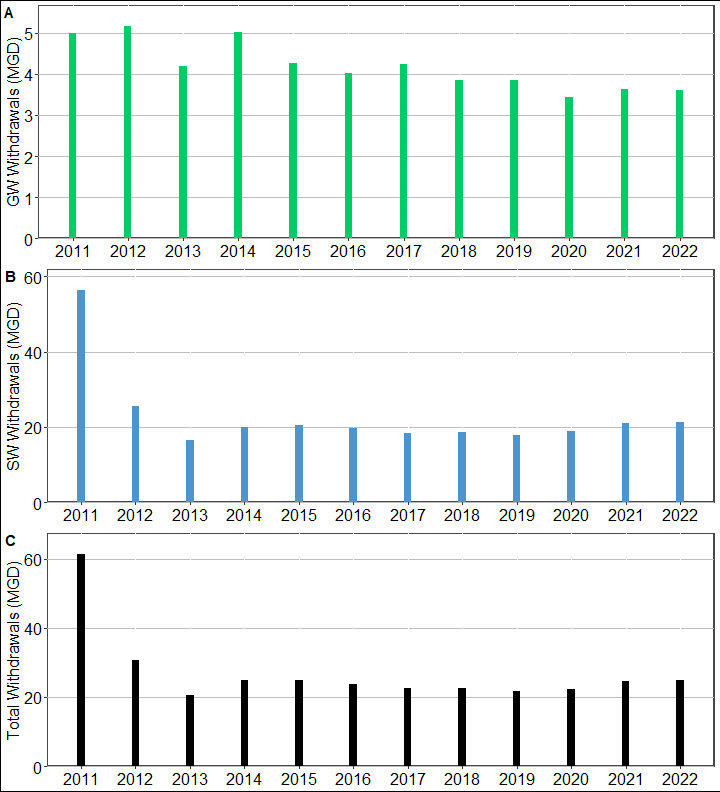
\includegraphics{LSS_figures/trend-IN_bar-plot-1} 

}

\caption{\textbf{Figure A5.} Annual water withdrawals in the Lower Savannah-Salkehatchie basin for Industry by source. Groundwater (GW) \textbf{(A)}, Surface Water (SW) \textbf{(B)}, and Total \textbf {(C)}.}\label{fig:trend-IN_bar-plot}
\end{figure}

\hypertarget{a.7-water-withdrawal-for-agriculture}{%
\subsection{A.7 Water Withdrawal for
Agriculture}\label{a.7-water-withdrawal-for-agriculture}}

\begin{figure}[H]

{\centering 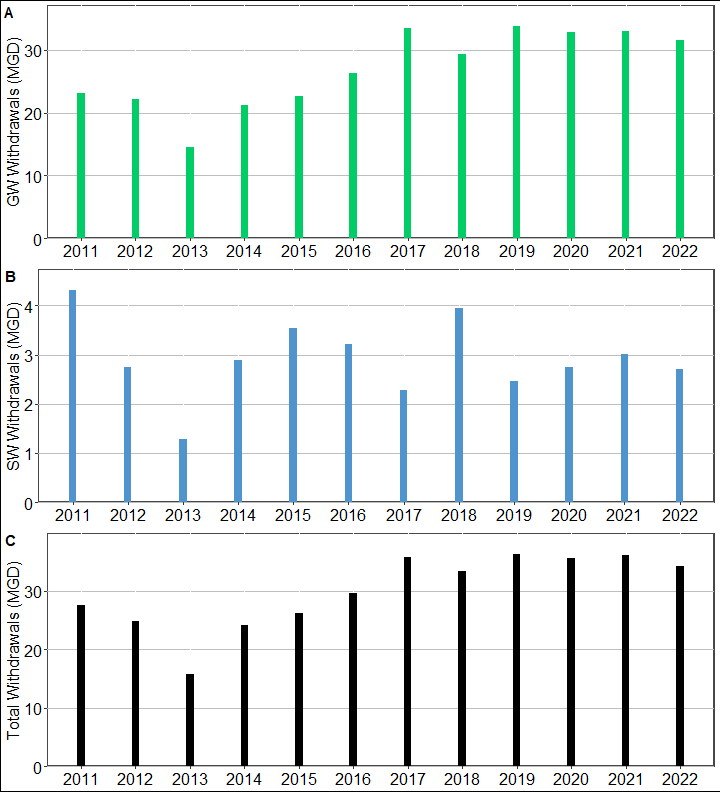
\includegraphics{LSS_figures/trend-Ag_bar-plot-1} 

}

\caption{\textbf{Figure A6.} Annual water withdrawals in the Lower Savannah-Salkehatchie basin for Agriculture by source. Groundwater (GW) \textbf{(A)}, Surface Water (SW) \textbf{(B)}, and Total \textbf {(C)}.}\label{fig:trend-Ag_bar-plot}
\end{figure}

\hypertarget{a.8-water-withdrawal-for-golf-course}{%
\subsection{A.8 Water Withdrawal for Golf
Course}\label{a.8-water-withdrawal-for-golf-course}}

\begin{figure}[H]

{\centering 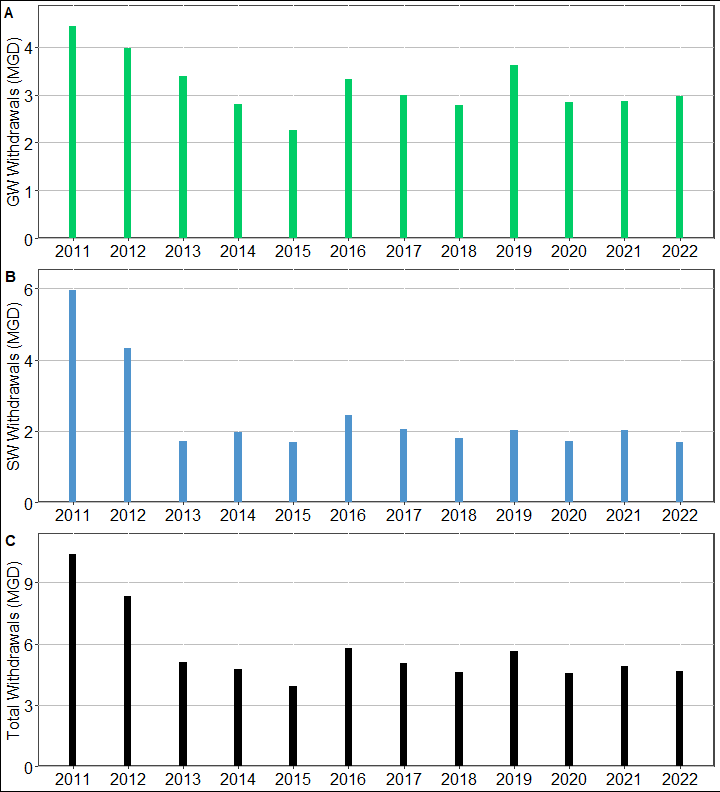
\includegraphics{LSS_figures/trend-GC_bar-plot-1} 

}

\caption{\textbf{Figure A7.} Annual water withdrawals in the Lower Savannah-Salkehatchie basin for Golf Course by source. Groundwater (GW) \textbf{(A)}, Surface Water (SW) \textbf{(B)}, and Total \textbf {(C)}.}\label{fig:trend-GC_bar-plot}
\end{figure}

\hypertarget{a.9-water-withdrawal-for-mining}{%
\subsection{A.9 Water Withdrawal for
Mining}\label{a.9-water-withdrawal-for-mining}}

\begin{figure}[H]

{\centering 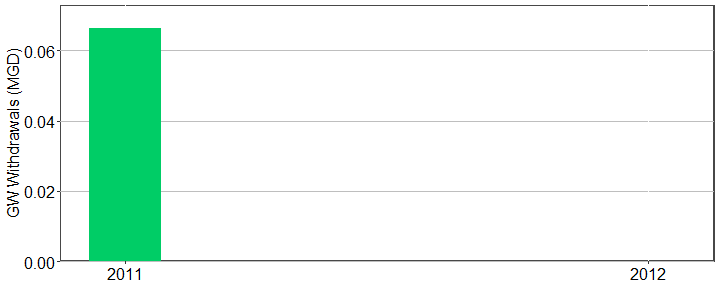
\includegraphics{LSS_figures/trend-MI_bar-plot-1} 

}

\caption{\textbf{Figure A8.} Annual groundwater (GW) withdrawals in the Lower Savannah-Salkehatchie basin for Mining.}\label{fig:trend-MI_bar-plot}
\end{figure}

\hypertarget{a.10-water-withdrawal-for-aquaculture}{%
\subsection{A.10 Water Withdrawal for
Aquaculture}\label{a.10-water-withdrawal-for-aquaculture}}

\begin{figure}[H]

{\centering 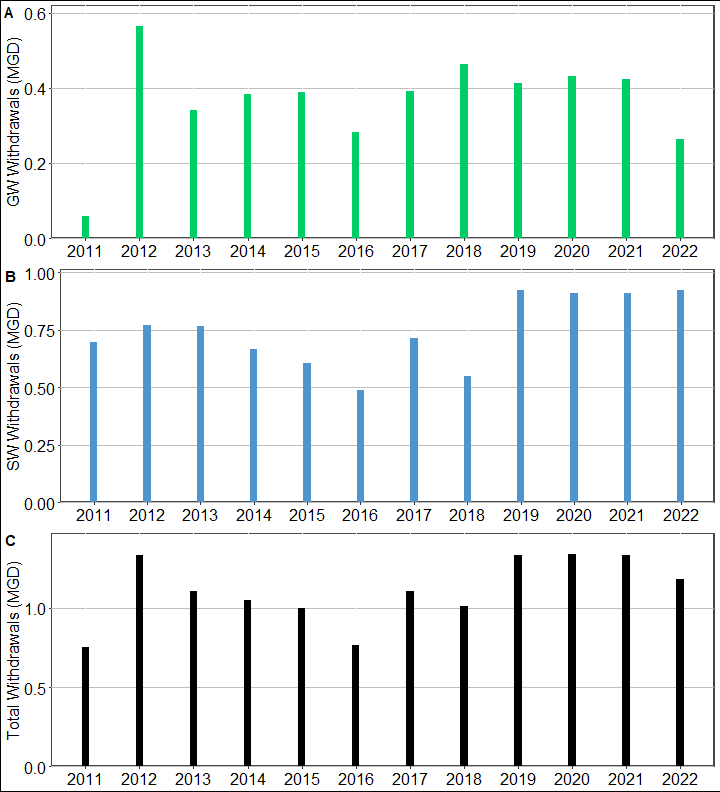
\includegraphics{LSS_figures/trend-AQ_bar-plot-1} 

}

\caption{\textbf{Figure A9.} Annual water withdrawals in the Lower Savannah-Salkehatchie basin for Aquaculture by source. Groundwater (GW) \textbf{(A)}, Surface Water (SW) \textbf{(B)}, and Total \textbf {(C)}.}\label{fig:trend-AQ_bar-plot}
\end{figure}

\hypertarget{a.11-water-withdrawal-for-other}{%
\subsection{A.11 Water Withdrawal for
Other}\label{a.11-water-withdrawal-for-other}}

\begin{figure}[H]

{\centering 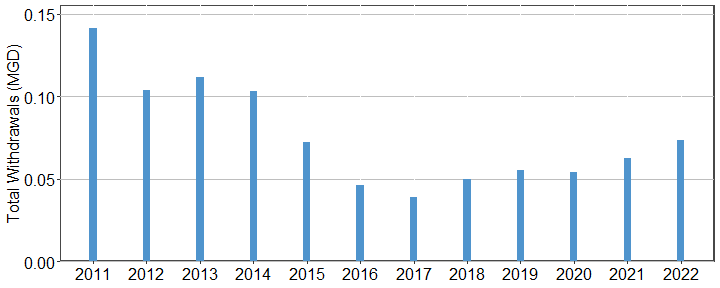
\includegraphics{LSS_figures/trend-OT_bar-plot-1} 

}

\caption{\textbf{Figure A10.} Annual groundwater (GW) withdrawals in the Lower Savannah-Salkehatchie basin for Other category.}\label{fig:trend-OT_bar-plot}
\end{figure}

\newpage

\hypertarget{references}{%
\subsection{References}\label{references}}

\begin{enumerate}
\def\labelenumi{\arabic{enumi}.}
\item
  Craig,B., and Monroe,L.A., 2020, South Carolina Department of Health
  and Environmental Control (SCDHEC) Water Use Report, 87
  p.~(\url{https://scdhec.gov/surface-groundwater-annual-water-use-report})
\item
  Wachob, A., Park, D.A., and Newcome R.Jr., 2009, South Carolina State
  Water Assessment, second edition: South Carolina Department of Natural
  Resources, 408 p.
  (\url{https://hydrology.dnr.sc.gov/pdfs/assessment/SC_Water_Assessment_2.pdf})
\end{enumerate}

\end{document}
